\documentclass[11pt]{article}

\usepackage[utf8]{inputenc}
\usepackage[T1]{fontenc}
\usepackage{lmodern}
\usepackage[margin=1in]{geometry}
\usepackage{graphicx}
\usepackage{booktabs}
\usepackage{amsmath}
\usepackage{siunitx}
\usepackage{caption}
\usepackage{authblk}
\usepackage[hidelinks]{hyperref}
\usepackage[numbers,sort&compress]{natbib}
\usepackage{microtype}
\usepackage{xcolor}

\captionsetup{font=small,labelfont=bf}
\graphicspath{{figures/}}

\title{\bfseries When Does the Model Look It Up?\\
Parametric Knowledge, Controlled Retrieval, and the\\ Mechanics of AI Answer Engines}

\author[ ]{Homiere Research}
\affil[ ]{\normalsize \texttt{hello@homiere.com}}
\date{July 2026}

\begin{document}
\maketitle

\begin{abstract}
\noindent
Large language models increasingly answer questions by combining what they learned in
pre-training with what they retrieve at query time. For any business that wants to be
recommended by these systems, the practical question is which of the two is decisive, and
whether the retrieval layer can be influenced. We study this with a controlled instrument:
Claude, served through AWS Bedrock with a \texttt{web\_search} tool whose results we author in
full. This lets us hold the evidence set fixed and vary, independently, (i)~how familiar the
model is with an entity (measured rather than assumed) and (ii)~what the retrieved documents
say. We construct three familiarity tiers - well-known national brands, real but obscure local
businesses, and fictitious entities - and confirm the tiers by probing the model with no search
access before any conflict trial. We find that a single controlled document overrides a
well-known brand's correct founding facts 93\% of the time; that providing documents converts
near-universal refusal about unknown entities (18 of 19) into 92--93\% adoption of whatever we
plant (McNemar $p = 7.6\times10^{-6}$); and that familiarity suppresses adoption of \emph{novel}
claims about a known entity (37\% vs.\ 92--93\% for unknown entities) even as it barely dents
\emph{corrective} claims (95\%). The model searches an order of magnitude harder for entities it
knows (11--16 \texttt{web\_search} queries vs.\ one or two). In a companion content-feature ablation
with retrieval held fixed, the model reorders candidates almost independently of the presented order
(Kendall's $\tau = 0.10$), and statistics, quotations, or authority markers each move a target from
mid-pack to first in every trial, from any position. We draw out the implications for
answer-engine optimization (AEO): establishing an unknown entity is a retrieval problem while
optimizing a known one is a content problem, the highest-leverage lever in both is dense
persuasive content, and the same features that constitute legitimate optimization also constitute
a cheap, uncritically trusted manipulation.
\end{abstract}

\section{Introduction}

An answer from claude.ai or ChatGPT that names three brokerages worth calling is not a single
act. It is the composition of at least three subsystems: the model's parametric memory laid down
in pre-training, a retrieval layer that issues searches and fetches pages, and the in-context
synthesis that turns retrieved text into an ordered recommendation. The optimization discipline
that has grown up around these systems (variously called ``AEO'' or ``GEO'') mostly reasons about the
composed behavior from the outside, and its practitioners disagree about the most basic mechanism.
One camp holds that the model largely relays the search engine's ranking, so the work that matters
is ordinary SEO. The other holds that the model curates, reweighting and filtering and sometimes
overriding what retrieval surfaces, so there is a distinct set of levers to pull. The disagreement
persists because it is hard to settle from observational data: on a live portal, retrieval and
generation are confounded, and a page may appear in an answer because the search backend ranked it
first, not because the model preferred it.

We remove the confound by controlling the evidence. Our subject model is Claude on AWS Bedrock,
invoked through the Converse API with tool use. We give it a \texttt{web\_search} tool with the
ordinary shape - a query in, ranked results out - but every result comes from a corpus we wrote.
Because the retrieval layer is now a fixed, known quantity, differences in the model's answers are
attributable to the two things we manipulate: the model's prior familiarity with the entity in
question, and the content of the documents it retrieves.

This paper reports the first phase of that program, which targets the prior-versus-evidence
question directly. We ask four things. First, does the model's pre-trained knowledge determine what
it says when search is available, or does controlled evidence take over? Second, when the evidence
contradicts a fact the model demonstrably knows, which one wins, and does that depend on how
well-known the entity is? Third, for entities the model has never heard of, the situation of
essentially every small business, does providing our documents convert an ``I'm not familiar with
them'' refusal into a confident, specifics-laden answer? Fourth, what does the model \emph{do} with
the tool: how often does it search at all, and what does it search for?

Our contribution is methodological as much as empirical. Prior knowledge-conflict work almost
always injects evidence directly into the prompt; we route it through a search tool the model must
choose to call, which is the actual deployment shape and lets us observe search behavior as an
outcome. Prior work also assumes entity familiarity from popularity proxies; we measure it per
entity on the subject model itself, and we show the measurement is necessary: it catches
name-collision cases where a ``well-known'' label is wrong. The result is a design in which every
factor that matters for AEO is either controlled or measured.

\section{Related Work}

\paragraph{Knowledge conflict.}
A now-substantial line of work \citep[surveyed by][]{xu2024knowledge} studies how models arbitrate
between parametric memory and
in-context evidence. \citet{longpre2021entity} introduced entity-substitution conflicts and found
models often ignore contradicting context in favor of memorized answers; \citet{xie2024adaptive}
showed much of that apparent stubbornness was an artifact of incoherent substituted passages, and
that with coherent evidence models are highly persuadable but show confirmation bias under mixed
evidence. \citet{wu2024clasheval} quantified the opposite failure - frontier models abandoning a
correct prior for incorrect retrieved content in a large fraction of cases - and demonstrated a
dose--response relationship between how implausible the evidence is and how often it is rejected.
\citet{kortukov2024studying} found that with realistic corrective documents, retention of a wrong
prior nearly vanishes, but that the model's own prior answer, if present anywhere in context,
raises the chance of an update failure. We adopt this literature's core dependent
variables (adoption, persistence, abstention) but move the evidence behind a search tool and add
measured familiarity as a first-class factor.

\paragraph{Entity popularity and parametric knowledge.}
\citet{mallen2023trust} established that factual recall tracks entity popularity and that retrieval
helps most below a popularity threshold; \citet{du2024context} formalized context susceptibility
and found it higher for fabricated than for real entities. These motivate our three-tier design,
but where that work uses popularity proxies and open models with log-probabilities, we screen
familiarity directly on the deployed model.

\paragraph{GEO/AEO.}
\citet{aggarwal2024geo} formalized generative engine optimization, reporting that adding
statistics, quotations, and citations to a source raised its share of the generated answer by up to
${\sim}40\%$ in a simulated engine, while keyword stuffing did nothing. Subsequent benchmarks have
contested how well these gains survive competition and how they transfer across engines
\citep{puerto2025cseo}. \citet{pfrommer2024ranking} is closest to our instrument: they load a fixed
set of real product pages into context and decompose ranking into brand-name prior, document
content, and position; the position sensitivity they and \citet{liu2024lost} document is what our
Experiment~2 controls for by construction. Our content-feature experiment sits in this line; the
present phase isolates the familiarity and evidence factors that GEO studies hold implicit. A full
annotated bibliography with verified citations accompanies the code release.

\section{Instrument and Methods}

\subsection{Model access}
All model calls go through the AWS Bedrock Converse API, which exposes a uniform tool-use interface
across Claude versions. The subject model for the results below is Claude Sonnet~4.5. Every request
and response (model id, decoding parameters, the full message transcript, each tool call and its
returned documents, and token usage) is logged verbatim to JSONL with the repository commit hash,
so any number in this paper can be traced to the exact interaction that produced it.

\subsection{The controlled search tool}
The model is offered a single tool, \texttt{web\_search}, described generically (``Search the web.
Returns the most relevant pages for a query''). Behind it is a lexical index over an authored
corpus: the model issues a natural-language query, the index returns the top-$k$ documents by
IDF-weighted overlap, formatted as title/URL/content blocks that mimic a real tool result. The
corpus is small and hand-built because the point is control, not retrieval quality. The index
records every query the model issues and which documents it served, so search behavior is itself
measured. When the model exhausts a fixed tool-call budget while still searching, we issue one
final call without tools so it must answer from what it has gathered, mirroring how production
answer engines cap tool use; trials where this occurred are flagged.

\subsection{Familiarity tiers, measured not assumed}
We define three tiers. \textbf{HIGH}: well-known national real-estate and home-services brands
(Redfin, Zillow, Keller Williams, Angi, Thumbtack, Opendoor, TaskRabbit). \textbf{TAIL}: real but
obscure small businesses - independent brokerages, boutique property managers, local inspectors,
movers, and stagers in small and mid-size metros - found and verified to have live websites via web
search. \textbf{ZERO}: fictitious entities we invented.

Tier membership is a hypothesis until confirmed. In a screening phase, each candidate is probed five
times, with no search access, at temperature~1, with a neutral prompt asking what the model knows
about it. A judge model scores each answer for the specificity of its claims (0--2) and whether it
disclaims familiarity. We classify an entity KNOWN if mean specificity $\geq 1.3$ with a low
disclaim rate, UNKNOWN if specificity $\leq 0.5$ with a high disclaim rate, and AMBIGUOUS otherwise,
and we keep only entities whose measured class matches their intended tier.

The screening confirmed 26 of 28 candidates into clean tiers: 7~HIGH (mean specificity 2.0, zero
disclaimers), 8~ZERO and 11~TAIL (specificity ${\approx}0$, near-universal disclaimers). All eight
fictitious entities showed zero leakage: none elicited any specific claim, validating them as
zero-knowledge controls. Two candidates were correctly rejected, both for the same reason: the
\emph{name} carried knowledge the \emph{entity} did not. ``Compass'' collides with several
well-known companies and triggered disambiguation rather than recall; a second candidate, a small
moving company, was rejected because its name incorporates a historical nickname for its home city,
which the model recognized independently of the business itself. These cases are the argument for
measuring familiarity rather than assuming it.

\subsection{Evidence treatments}
For each entity we author documents under up to three treatments. \textbf{Novel} (all tiers):
documents assert specific facts the model could not already know - a distinctively named program,
precise statistics, named people, a founding year. For fictitious and tail entities these invented
specifics are the only facts available; for HIGH brands they are a plausible recent (2025--26)
development. Adoption of these facts is the primary signal that controlled evidence entered the
answer. \textbf{Consistent} (HIGH only): a document that restates the model's true prior facts plus
one benign new detail - a no-conflict control. \textbf{Contradicting} (HIGH only): documents that
confidently assert false versions of two facts the model demonstrably knows (a wrong founding year
and a wrong founding city or founder). Here the planted false claims are the adoption probes and the
true facts are the persistence probes; ``evidence wins'' means the model asserted the false planted
fact and not the true one. Each trial's search index contains the treatment's documents plus shared
generic distractors, so retrieval always returns competition.

\subsection{Outcomes and scoring}
Each trial is scored by an LLM judge that decides, for every probe, whether the answer asserts it,
contradicts it, or is silent; a separate rule-based detector flags whether the answer abstains
(declines for lack of information). This replaces the brittle
string-matching used in piloting, which missed obvious paraphrases (``\textbf{Founded:} 2002'' does
not contain the substring ``founded in 2002''). From these we compute, per cell: adoption rate
(fraction of a treatment's planted facts asserted), prior-persistence rate (fraction of true facts
retained under contradiction), abstention rate, and the number and content of search queries issued.

\subsection{Analysis}
Primary estimates are at temperature~0; we report tier~$\times$~treatment means with 95\% bootstrap
confidence intervals resampled over entities, a McNemar test on the abstention flip between the
no-search and search conditions, and a logistic model of fact-level adoption on tier and treatment
clustered on entity. Hypotheses and analysis code were committed before the confirmatory runs.

\section{Results}

\subsection{Prior versus controlled evidence (Experiment~1)}
The full run comprised 66 trials at temperature~0 with no empty answers; adoption and persistence
were scored by the judge, and confidence intervals are bootstrap resamples over entities.
Table~\ref{tab:exp1} and Figure~\ref{fig:adoption} summarize the adoption results.

\begin{table}[t]
\centering
\caption{Experiment~1: adoption of planted facts and prior persistence by familiarity tier and
evidence treatment (temperature~0). Adoption is the fraction of a treatment's planted facts the
answer asserts; for the no-search baseline rows, which have no documents, it is the base rate at
which the model asserts the would-be-planted (novel) facts unaided - the comparison point for the
novel treatment. Persistence is the fraction of true prior facts retained under a contradicting
document (defined only for the HIGH tier, which alone has a prior to contradict).}
\label{tab:exp1}
\small
\begin{tabular}{llS[table-format=1.2]cS[table-format=1.2]}
\toprule
Tier & Treatment & {Adoption} & {95\% CI} & {Prior persistence} \\
\midrule
HIGH & no-search baseline (prior) & 0.36 & [0.31, 0.42] & {1.00} \\
HIGH & consistent (agrees with prior) & 0.96 & [0.89, 1.00] & {--} \\
HIGH & contradicting (false core facts) & 0.95 & [0.86, 1.00] & {0.07} \\
HIGH & novel (new program/stat) & 0.37 & [0.19, 0.57] & {--} \\
TAIL & no-search baseline (prior) & 0.00 & [0.00, 0.00] & {--} \\
TAIL & novel & 0.92 & [0.87, 0.96] & {--} \\
ZERO & no-search baseline (prior) & 0.00 & [0.00, 0.00] & {--} \\
ZERO & novel & 0.93 & [0.86, 0.98] & {--} \\
\bottomrule
\end{tabular}
\end{table}

\begin{figure}[t]
\centering
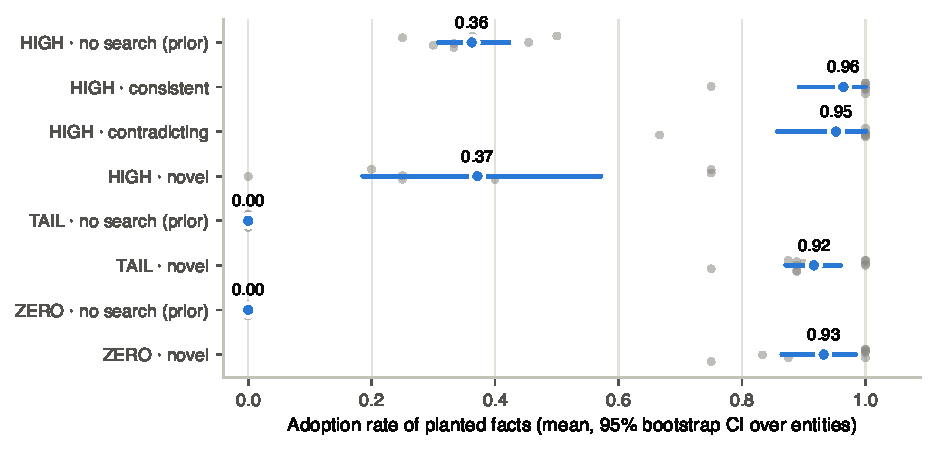
\includegraphics[width=0.92\linewidth]{fig_adoption.pdf}
\caption{Adoption of planted facts by tier and treatment. Dots are per-entity trials (jittered);
the marker is the mean and the bar its 95\% bootstrap confidence interval over entities. Controlled
evidence is adopted near-universally except for \emph{novel} claims about \emph{known} (HIGH)
entities, where the model is markedly more skeptical.}
\label{fig:adoption}
\end{figure}

\paragraph{Controlled evidence overrides a well-known brand's correct facts.}
With no search, the seven HIGH-familiarity brands state their true founding facts (baseline
persistence 1.00). Given one authored page asserting a false founding year and city, the model
adopted the false version 95\% of the time (95\% CI [0.86, 1.00]) and retained the truth only 7\% of
the time; controlled evidence won roughly 93\% of the conflicts. The effect holds for
household-name brands (Redfin, Zillow, Keller Williams), not only obscure entities, replicating the
ClashEval-style override phenomenon \citep{wu2024clasheval} on a current Claude model through a
search tool rather than prompt injection.

\paragraph{Search converts refusal into confident assertion for unknown entities.}
Without search, unknown entities are refused (ZERO abstains 100\%, TAIL 91\%). With our documents
available, abstention collapses to zero and the model asserts 92--93\% of whatever facts we planted
(ZERO 0.93 [0.86, 0.98]; TAIL 0.92 [0.87, 0.96]). Across the 19 unknown entities, 18 refused without
search and none did with it (McNemar exact $p = 7.6\times10^{-6}$). For an entity outside the
training corpus - essentially every small business - the retrieved document is, in effect, the
model's knowledge.

\paragraph{Familiarity breeds skepticism of novel claims but not of corrective ones.}
Novel claims - a plausible new 2025--26 program or statistic - were adopted only 37\% of the time for
HIGH brands [0.19, 0.57] versus 92--93\% for TAIL and ZERO. In the fact-level logistic model
(clustered on entity), being TAIL or ZERO adds $+1.45$ / $+1.53$ to the log-odds of novel adoption
(both $p < 0.001$). Yet those same HIGH brands adopted \emph{contradictions of their core facts} at
95\%. The model resists \emph{adding} surprising new attributes to an entity it knows while readily
\emph{overwriting} the core attributes it knows; skepticism attaches to novelty about a known
entity, not to conflict as such.

\paragraph{Prior knowledge governs search effort.}
Search intensity separated the tiers by an order of magnitude (Figure~\ref{fig:search}): HIGH
entities drew 11--16 tool queries per trial (up to 22; 57\% of HIGH-novel trials exhausted the tool
budget), while TAIL and ZERO drew 1.2--1.5. The model interrogates the evidence hardest exactly when
a novel claim conflicts with a strong prior. Search effort is thus a direct function of prior
familiarity: the model is not a passive relay.

\begin{figure}[t]
\centering
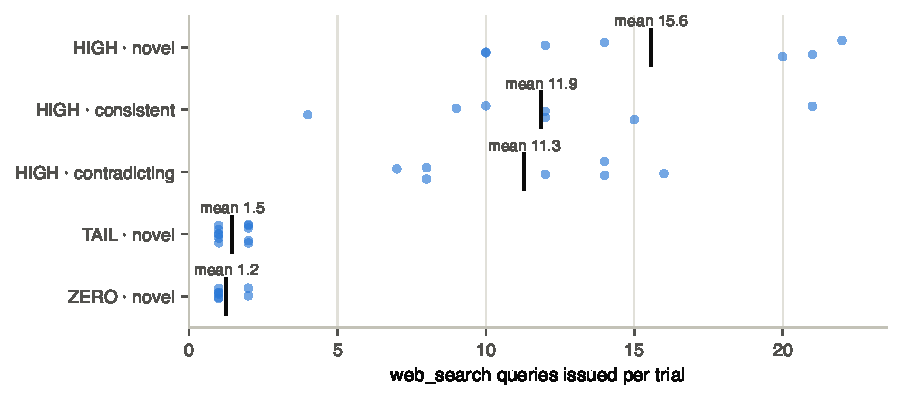
\includegraphics[width=0.92\linewidth]{fig_search.pdf}
\caption{Search intensity in the search condition. Each dot is one trial; the vertical rule is the
cell mean. The model issues an order of magnitude more \texttt{web\_search} queries for entities it
knows (HIGH) than for those it does not (TAIL, ZERO), and most of all when a novel claim conflicts
with a strong prior.}
\label{fig:search}
\end{figure}

\subsection{Content features and the curation rate (Experiment~2)}
Ninety trials (temperature~0 plus two replicates) over five comparable fictitious realtor CRMs; the
target's page was rewritten under content-matched feature treatments and its position rotated across
all five result slots with a fixed-order tool, so position is controlled.

\paragraph{The model curates rather than relays (AEO $\neq$ SEO).}
The mean Kendall's $\tau$ between the presented result order and the model's ranking was 0.10, near
zero (Figure~\ref{fig:tau}). The model reorders the candidates almost independently of the order
they were presented in, deciding rank from content. Being first in the result set buys little if a
competitor's page is more persuasive.

\paragraph{Statistics, quotations, and authority markers each take a product from mid-pack to
first in every trial, from any position.}
Each of these three content-matched rewrites moved the target from a baseline mean rank of 3.4
(never first) to a mean rank of 1.0 (first in every trial), regardless of presented position
(Figure~\ref{fig:heatmap}). Presented \emph{last}, the authority-marked page was still ranked first,
with the model citing the (fabricated) award and certification as its reason. Recency cues produced
a strong but partial effect (rank 1.8, first 60\% of the time). This aligns in direction with GEO's
finding \citep{aggarwal2024geo} that statistics, quotations, and citations are the strongest levers,
and extends it to a competitive ranking with position held fixed.

\paragraph{FAQ formatting hurts, independent of content (Experiment~2b).}
In the main run the FAQ-formatted target ranked worst, but that treatment was
confounded: the Q\&A rewrite also thinned the feature claims. We therefore re-ran with content held
constant across four target variants (Figure~\ref{fig:faq}). With the \emph{full} feature set, plain
prose ranked first in every trial (mean rank 1.0) while the same content as an FAQ ranked 4.4 of 5;
the FAQ version was if anything longer (132 vs.\ 99 words), so length does not explain the gap. The
mechanism is visible in the model's rationale: on the prose page it wrote ``comprehensive feature
set,'' and on the Q\&A version of the identical facts ``the most bare-bones option\ldots lacks
standout features.'' Two effects separate cleanly and both are real: fuller content helps (prose
with the full feature set beat prose with a partial set, 1.0 vs.\ 3.6), and the Q\&A format itself
hurts (${\sim}3.4$ rank positions at matched content). Structured markup for direct-answer
extraction is one thing; on a ``which should I choose'' query, formatting the page as an FAQ made the
model read it as less substantial.

\begin{figure}[t]
\centering
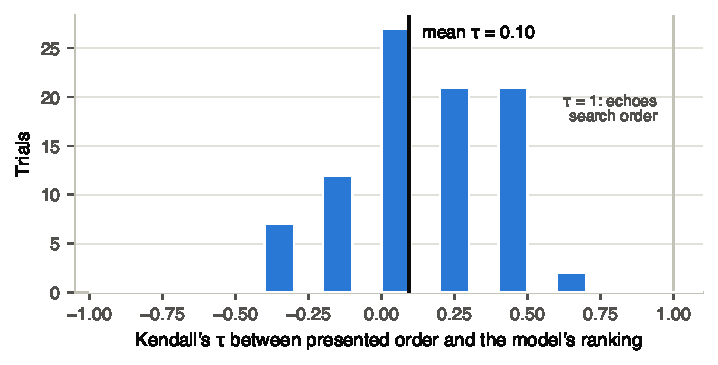
\includegraphics[width=0.78\linewidth]{fig_tau.pdf}
\caption{Distribution of the curation rate: Kendall's $\tau$ between the presented (search) order
and the model's ranking, over 90 trials. A relay would concentrate near $\tau=1$; the observed mean
of 0.10 shows the model reorders on content, largely ignoring presented position.}
\label{fig:tau}
\end{figure}

\begin{figure}[t]
\centering
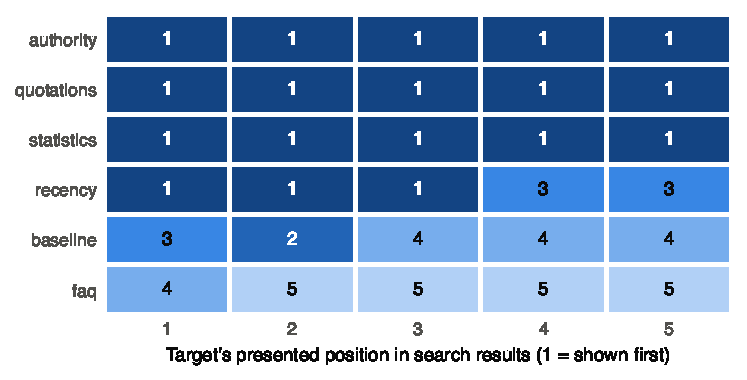
\includegraphics[width=0.78\linewidth]{fig_rank_heatmap.pdf}
\caption{Experiment~2: the target product's rank (1~=~best of 5; darker~=~better) by content-feature
treatment and by the position at which it was presented in the search results. Statistics,
quotations, and authority each secure first place from every position; recency helps partially;
baseline and FAQ do not. Position (columns) has little effect within a treatment.}
\label{fig:heatmap}
\end{figure}

\begin{figure}[t]
\centering
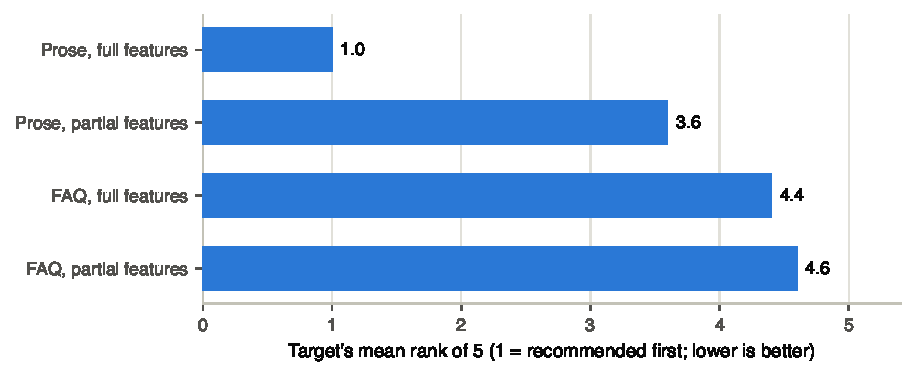
\includegraphics[width=0.86\linewidth]{fig_faq.pdf}
\caption{Experiment~2b: target mean rank (1~=~recommended first of 5; lower is better) with content
held constant. The identical full feature set ranks first in prose but 4.4 of 5 as an FAQ; the same
partial set is worse in both formats. The prose/FAQ gap at full content isolates the format effect.}
\label{fig:faq}
\end{figure}

\section{Discussion}

Two pictures of the answer engine are often posed as alternatives: a relay that repeats the search
ranking, and a curator that reweights it. Our results say it is both, and which one dominates is
governed by entity familiarity. For entities the model has never seen, it searches barely, does not
curate against a prior it does not have, and repeats what the retrieved document says - the relay
picture, and the reason getting \emph{found} is nearly sufficient for an unknown business to be
described authoritatively. For entities it knows, it curates hard: it searches ten times as much,
resists novel additions, and on comparative queries reorders candidates almost independently of the
presented order, driven by content features. The curation is real and it is large: three ordinary
content features each turned a mid-pack product into the first recommendation in every trial.

For AEO this reframes the problem by familiarity. Establishing an unknown entity is a retrieval
problem: be in the result set with a clear, specific, factually rich page, and the model will speak
to it. Optimizing a known entity is a content problem: the retrieval layer can still overwrite its
core facts, but novel claims about it are discounted and heavily verified, so credibility and
corroboration matter more. Across both regimes the highest-leverage move is the same - dense,
concrete, persuasive claims (statistics, testimonials, credible authority) rather than formatting
tricks or keyword density.

The manipulation boundary is visible already: the authority markers that
lifted the product to first were fabricated, and the model adopted and cited them without
skepticism. That the same features which constitute legitimate optimization also constitute a cheap
attack - the concern of a growing adversarial literature
\citep{kumar2024manipulating,nestaas2024adversarial} - is a central tension that warrants further
study. Situating these controlled findings against the production portals, in order to measure how
far a Bedrock reconstruction tracks claude.ai, ChatGPT, and the other scrapable surfaces, is a
natural direction for future work.

\section{Limitations}
\label{sec:limitations}

The controlled search tool is a faithful \emph{shape} of a real tool, not a real one; measuring the
gap between this instrument and the production portals directly, rather than assuming it away, would
require a separate portal-fidelity study. Results are for one model family (Sonnet~4.5) accessed
through Bedrock at temperature~0; system prompts and post-processing on the consumer portals are
opaque, and temperature-1 replicates for stability - answer visibility in these systems is better
characterized as a distribution over repeated runs than a point estimate \citep{schulte2026dont} - are
a queued extension. Familiarity is measured
on the subject model at one point in time, and production models drift. The abstention detector is
pattern-based and over-triggers on partial hedges (one HIGH case gave a complete answer but hedged
on a single sub-fact); the unknown-entity abstention flip involves unambiguous full refusals and is
unaffected. The Experiment~2b matched arms are content-matched but not exactly length-matched (the
Q\&A version is longer, which if anything works against the format-hurts finding). Experiment~2's
effect magnitudes come from a single product category and warrant replication across categories and
models. Fictitious and tail entities let us
plant facts freely, which is ideal for measurement but means the ``novel'' adoption results describe
behavior on unknown entities specifically.

\paragraph{Reproducibility.}
The code, authored corpora, raw model outputs (JSONL, one record per API interaction), analysis
scripts, and figure-generation code are released with this paper, and each result traces to a logged
interaction stamped with the repository commit hash. One exception: the raw inputs and outputs for
the tail tier are withheld from the public release, because that tier authored fabricated facts about
real, named small businesses and we do not wish to publish that association; the tier's aggregate
results (which name no business) are reported here, and the withheld data is available to researchers
on request. The well-known-brand and fictitious tiers are fully included.

\bibliographystyle{plainnat}
\bibliography{references}

\end{document}
